%% This is an example first chapter.  You should put chapter/appendix that you
%% write into a separate file, and add a line \include{yourfilename} to
%% main.tex, where `yourfilename.tex' is the name of the chapter/appendix file.
%% You can process specific files by typing their names in at the 
%% \files=
%% prompt when you run the file main.tex through LaTeX.

\singlespacing{

\chapter{Simulation of Function-Level Parts}\label{chap:functionSim}

Simulation of function-level parts is carried out through a mass/spring/damper model.  In this model, neighboring face-connected cells apply forces and torques on one another through local interactions.  Translational and rotational positions and velocities are calculated from these forces using discrete-time integration techniques.  Internal degrees of freedom of \textit{functions} are parameterized by 15 stiffness and damping coefficients, $k$ and $d$.  Actuation is achieved by modulating the nominal distance of adjacent cells along a particular degree of freedom.  %In a sense, this type of simulation could be thought of as a dynamic constraint-solving system between solid elements with various degrees of freedom.

\section{Existing Models of Solids}

Mass/spring/damper
FEA

%Unlike traditional mass/spring/damper models of solids from computer graphics literature (cite stuff here), the model developed in this thesis draws on an abstraction of the functionality embedded in the different "function types".

\begin{figure}
  \includegraphics[width=\linewidth]{SolidMechanicsDOF.png}
  \caption{Deformations of a solid element under four types of applied forces.  In modeling assemblies of \textit{functions}, these characteristic deformations are referred to as "internal degrees of freedom".}
  \label{fig:SolidMechanicsDOF}
\end{figure}

In solid mechanics, we can consider the global deformations of a solid as the summation of deformations of many smaller, discrete volumes, or \textit{finite elements}.  Forces acting on these finite elements fall into four categories: longitudinal (tension and compression), bending, shear, and torsion.  Each type of applied force causes a characteristic deformation of the finite element, indicated in Figure \ref{fig:SolidMechanicsDOF}.  Applying multiple types of forces on a finite element will cause it to exhibit a combination of deformations.\\

In this model, simulation of an assembly happens at the granularity of identically-sized \textit{function}-level parts, which we'll call "cells".  When describing mechanical behavior of a particular cell type, we refer to its deformations as "internal degrees of freedom" (DOF).  For example, a 1-DOF bending cell will have large deformations in bending along one axis, but relatively small deformations in response to other types of applied forces.\\

\section{Function Types}

Cells at the function-level are defined not only by their mechanical properties, but also by their ability to transmit electronic signals from one face to another, and their active properties in response to a signal. The combinatorial space of mechanical, electronic, and actuated cell types is described in Figure \ref{fig:CombinatoricsOfFunctions}.  Section \ref{sec:electronicSim} describes the process of electronic simulation in more detail, the remainder of this chapter will focus on the passive and active mechanical simulation of function-level cells.
\\

\begin{figure}
  \includegraphics[width=\linewidth]{CombinatoricsOfFunctions.png}
  \caption{Combinatorial space of function types.}
  \label{fig:CombinatoricsOfFunctions}
\end{figure}

\section{Geometric Stiffness}

The geometric stiffness of a structure relates the bulk properties of a material to its 3d geometry.  For example, an I-beam has a higher geometric bending stiffness than an equal length rectangular bar made from the same amount of the same material.  Unless otherwise noted, "stiffness" in this analysis refers to geometric stiffness.\\

Stiffness and damping are used to characterize the response of cell's internal degrees of freedom to applied external forces.  In three dimensions, each cell's passive mechanical properties are parameterized by 15 stiffness and damping constants:

\[ k =  \left\{ \begin{array}{ccc}
k_{longitudinal_x}\\
k_{ongitudinal_y}\\
k_{longitudinal_z}\\
\\
k_{shear_{xy}}\\
k_{shear_{xz}}\\
k_{shear_{yx}}\\
k_{shear_{yz}}\\
k_{shear_{zx}}\\
k_{shear_{zy}}\\
\\
k_{bending_x}\\
k_{bending_y}\\
k_{bending_z}\\
\\
k_{torsional_x}\\
k_{torsional_y}\\
k_{torsional_z}
 \end{array} \right\} 
 \qquad\qquad
 d =  \left\{ \begin{array}{ccc}
d_{longitudal_x}\\
d_{longitudal_y}\\
d_{longitudal_z}\\
\\
d_{shear_{xy}}\\
d_{shear_{xz}}\\
d_{shear_{yx}}\\
d_{shear_{yz}}\\
d_{shear_{zx}}\\
d_{shear_{zy}}\\
\\
d_{bending_x}\\
d_{bending_y}\\
d_{bending_z}\\
\\
d_{torsional_x}\\
d_{torsional_y}\\
d_{torsional_z}
 \end{array} \right\}  \]
\\

$k_{shear}$ and $d_{shear}$ are broken out into six parameters of the form $shear_{nm}$ because the shear response depends both on the direction of shear displacement between two cells ($m$) and on the axis along which the cells are connected ($n$).  The $shear_{nm}$ notion used above is described graphically in in Figure \ref{fig:ShearDOFs}.\\

\begin{figure}
  \includegraphics[width=\linewidth]{ShearDOFs.png}
  \caption{Illustration of shear subscript notation.  First subscript describes the direction of neighboring cell connection, second describes the direction of shear displacement.}
  \label{fig:ShearDOFs}
\end{figure}

The stiffness and damping constants of each \textit{function} type may be calculated from bulk properties of the constituent materials that make up a \textit{function}, or they may be measured empirically.  For example, an isotropic \textit{function} made from a bulk material with elastic modulus $E$ and shear modulus $G$ has stiffnesses defined by:

\[ k_{longitudinal} = \dfrac{aE}{l}\]
\[ k_{shear} = \dfrac{Ga}{l}\]
\[ k_{torsion} = \dfrac{GJ}{l}\]
\[ k_{bending} = \dfrac{aE}{l}\]
\\
where $a$ is the cross sectional area and $l$ is the length of the \textit{function}.\\

A linear scale showing the range of physically achievable 1-DOF bending \textit{function} types compared with the range of theoretically possible types is shown in Figure \ref{fig:BendingStiffnessContinuoum}.  Due to manufacturing and material constraints, we do not envision \textit{functions} that occupy the region near zero bending stiffness (e.g. a frictionless pin joint) or infinite bending stiffness.

\begin{figure}
  \includegraphics[width=\linewidth]{BendingStiffnessContinuoum.png}
  \caption{Continuum of bending stiffness in a 1 DOF hinge.}
  \label{fig:BendingStiffnessContinuoum}
\end{figure}


\section{Translational Forces}

\begin{figure}
  \includegraphics[width=\linewidth]{translationalSim.png}
  \caption{translationalSim.}
  \label{fig:translationalSim}
\end{figure}

%I started with a simple dynamic mechanical model where the forces acting on each cell in the lattice are computed based on local interactions with its six neighbors and gravity.  In the model, virtual springs and dampers constrain translational and rotational motion of a cell relative to its neighbors (Fig \ref{fig: helloWorldLocalInteraction}).  At each time step all forces acting on each cell in the lattice are summed and the position, orientation, and translational and rotational velocities of the cell are solved by Euler integration.  All cells are updated synchronously, so the order of evaluation of the cells is not important.  All physical constants used in these calculations (mass of the cell, moment of inertia, spring stiffness, damping coefficient) are derived from the geometry and material properties of each cell.\\
%
%In this scheme, the total force applied to the center of mass of a cell is given by:
%
%\[ F_{total} =  \vec{f}_g+ \sum_{neighbors} \vec{f}_{neighbor}\]
%
%With the total torque applied to the cell is given by the sum of the torques applied by its neighbors:
%
%\[ T_{total} =  \sum_{neighbors} \tau_{neighbor} \]
%
%
%\begin{figure}
%  \includegraphics[width=\linewidth]{helloWorldLocalInteraction.png}
%  \caption{REPLACE THIS Each cell is face-connected to its six local neighbors \textbf{(A)}.  Interaction between neighbors is modeled with springs and dampers constraining translational and rotational motion \textbf{(B)}.}
%  \label{fig: helloWorldLocalInteraction}
%\end{figure}
%
%%To understand how the translational spring forces were calculated between two adjacent cells, consider the 2D case illustrated in Fig \ref{fig: helloWorldSpringSetup}.  The cells are attached by a spring with nominal length $\ell$.  Under displacement $\Delta x$ and $\Delta y$, the distance vector from cell A to cell B is given by $\vec{D}$.  Then $\Delta \ell$, the displacement of the spring from its nominal length, is given by:\\
%%
%%\[ \Delta \ell = \| D\| - \ell\]
%%
%%The force, $\vec{f}_{AB}$, exerted on cell A by a spring with stiffness $k$ is oriented in the same direction as $\vec{D}$:
%%
%%\[ \vec{f}_{AB} =  k (\hat{D} \Delta \ell) = k\hat{D} (\|D\| - \ell)\]
%%
%%An equal and opposite force, $\vec{f}_{BA}$, is applied to cell B by the spring:
%%
%%\[ \vec{f}_{BA} = -k\hat{D} (\|D\| - \ell)\]
%%
%%\begin{figure}
%%  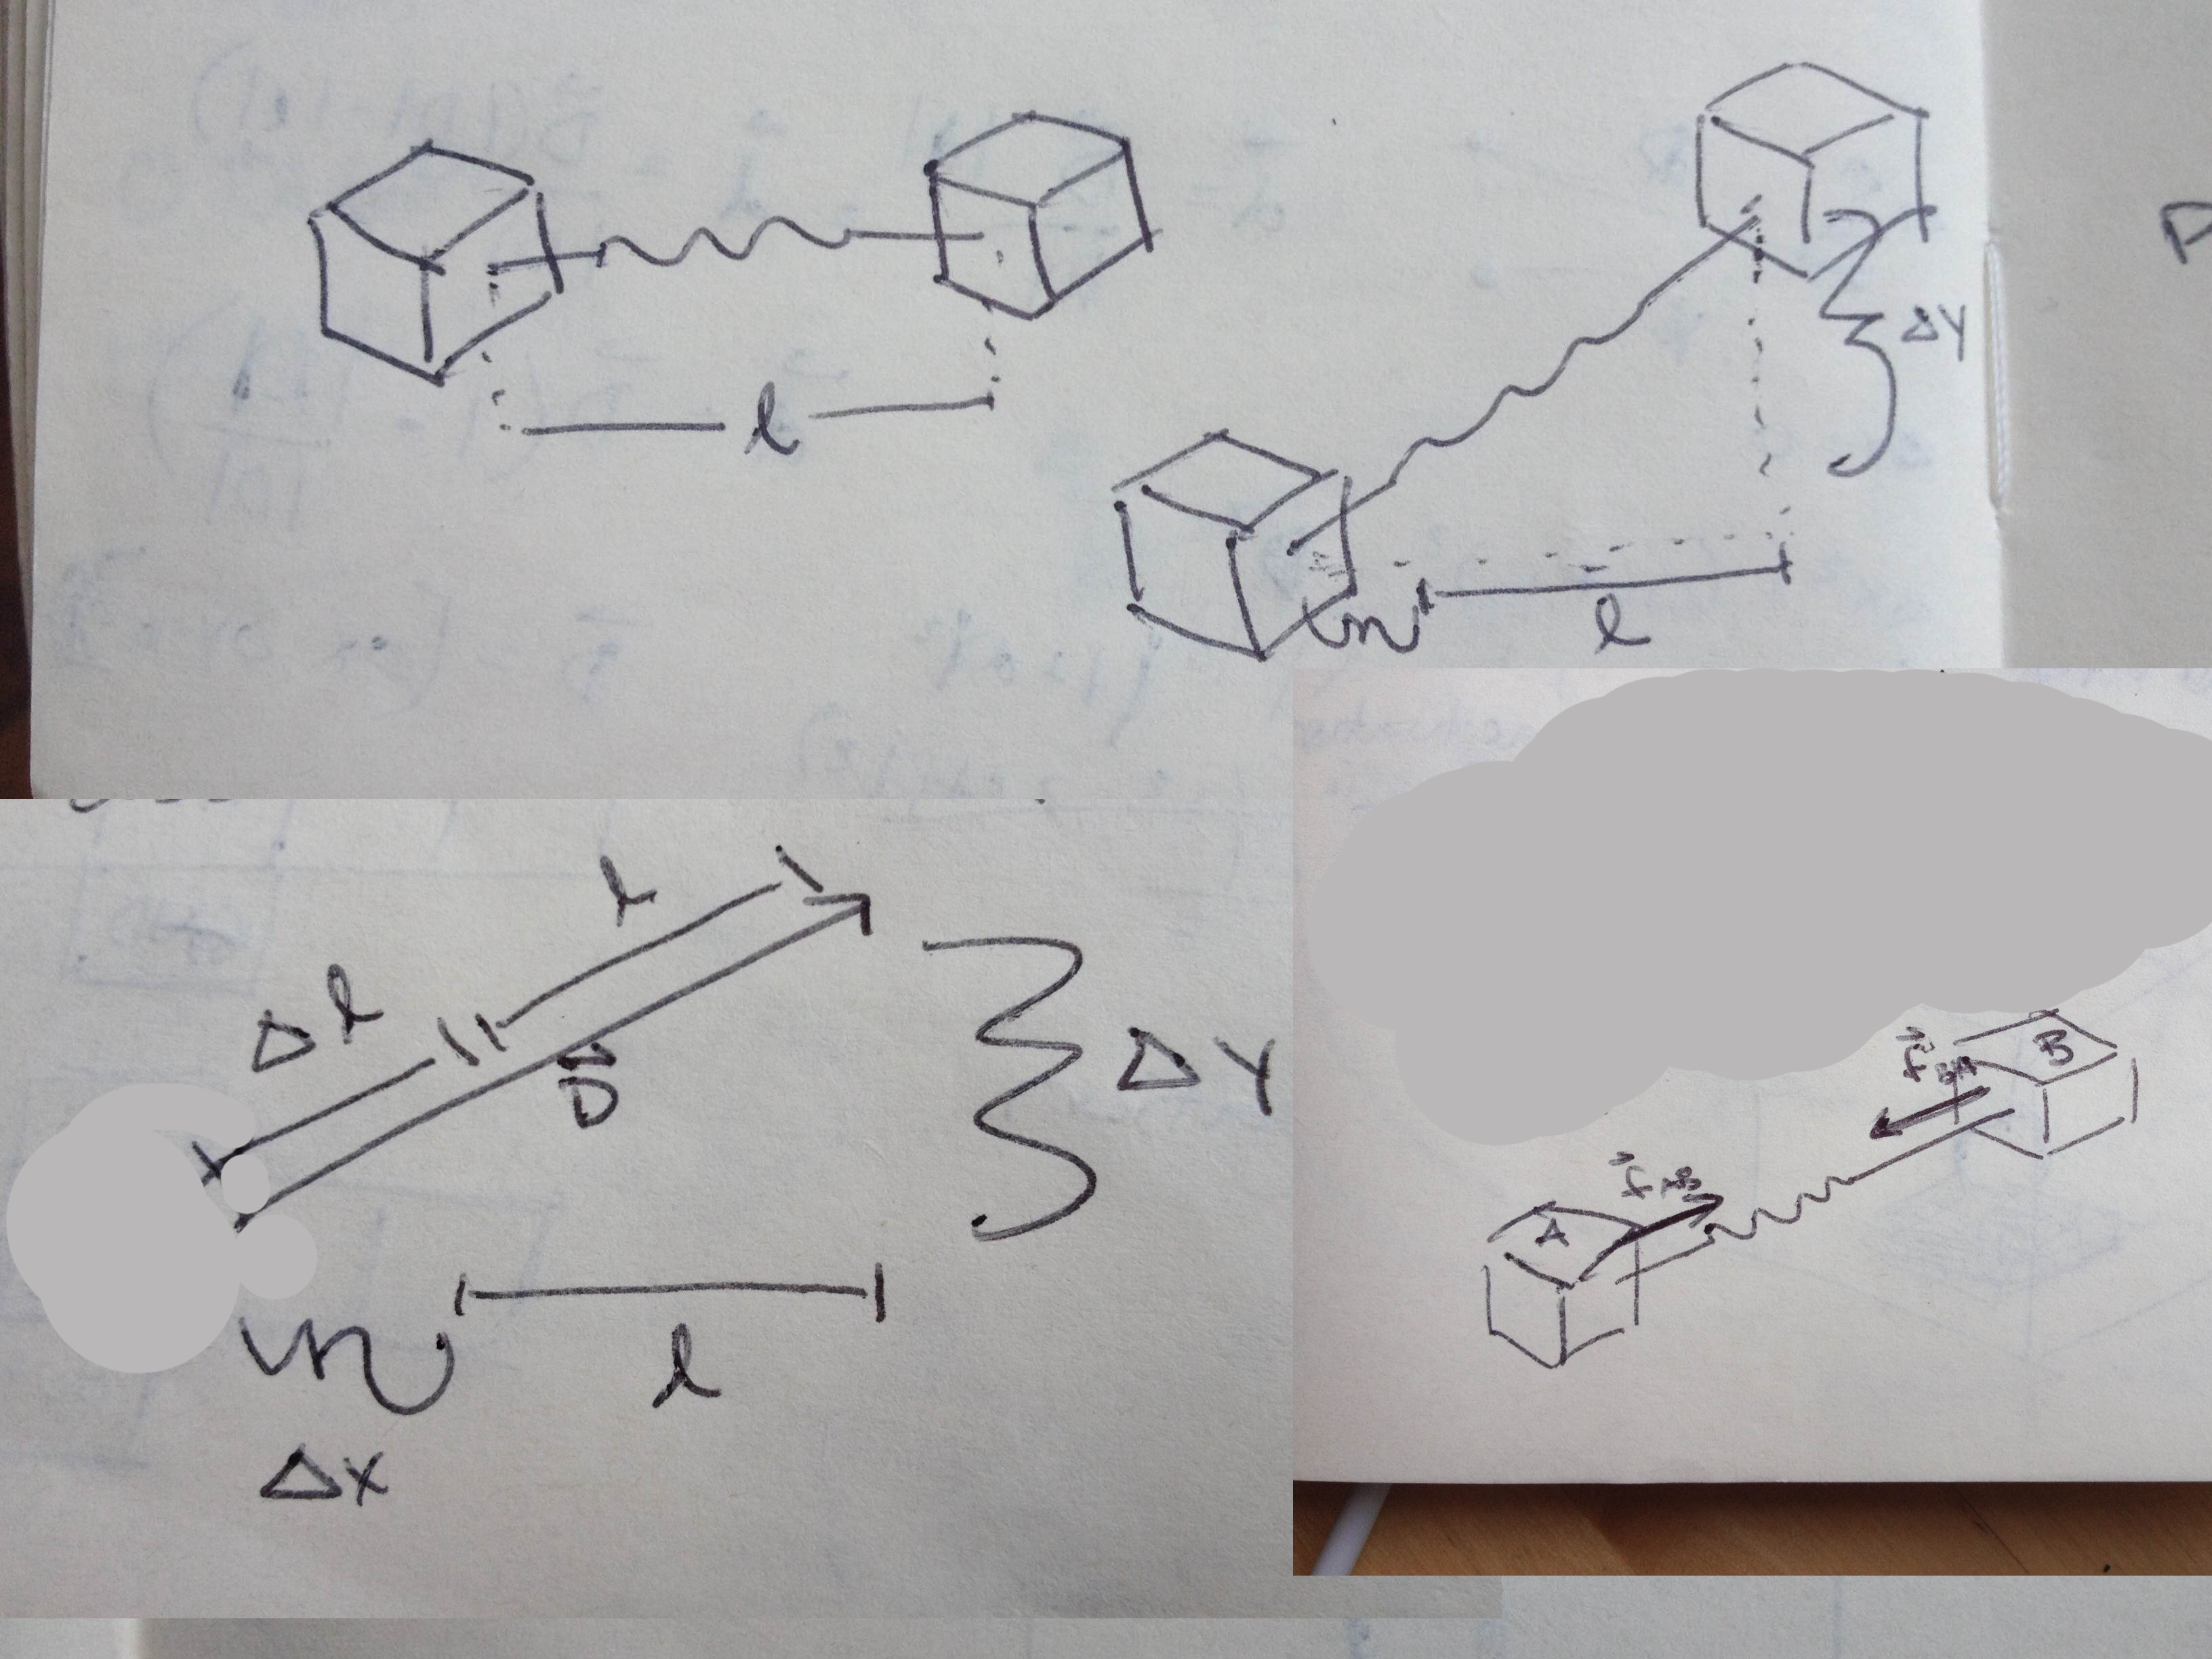
\includegraphics[width=\linewidth]{helloWorldSpringSetup.png}
%%  \caption{REPLACE THIS Cubes A and B connected by spring with nominal length $\ell$ \textbf{(A)}.  The cells are displaced by $\Delta x$ and $\Delta y$ \textbf{(B)}. Spring displacement $\Delta \ell$ along $\vec{D}$ \textbf{( C )}.  $\vec{f}_{AB}$ and $\vec{f}_{BA}$ are the resulting translational spring forces applied to cells A and B, respectively \textbf{(D)}.  Larger translational displacements between neighboring cells increase the amplitude of spring forces \textbf{(E)}.}
%%  \label{fig: helloWorldSpringSetup}
%%\end{figure}
%
%To understand how the translational forces were calculated between two adjacent cells, consider the 2D case illustrated in Fig \ref{fig: helloWorldSpringSetup}.  The cells are attached to each other with nominal displacement $\vec{\ell}$ from the center of cell A to the center of cell B.  If we model a two dimensional spring damper system connecting the cells, then the force applied to cell A by cell B under additional displacement $\Delta x$ and $\Delta y$ is given by:
%
%\[ \vec{f}_{AB} =   k\left[ \begin{array}{ccc}
%\Delta x \\
%\Delta y \end{array} \right] - d 
%\left[ \begin{array}{ccc}
%v_x\\
%v_y\end{array} \right] 
% \]
%
%where k is a spring stiffness, d is a damping coefficient, and $v$ is the velocity of cell A relative to cell B.  This equation is trivially extended to the three dimensional case:\\
%
%\[ \vec{f}_{AB} =   k\left[ \begin{array}{ccc}
%\Delta x \\
%\Delta y\\
%\Delta z \end{array} \right] - d 
%\left[ \begin{array}{ccc}
%v_x\\
%v_y\\
%v_z\end{array} \right] 
% \]
%
%\begin{figure}
%  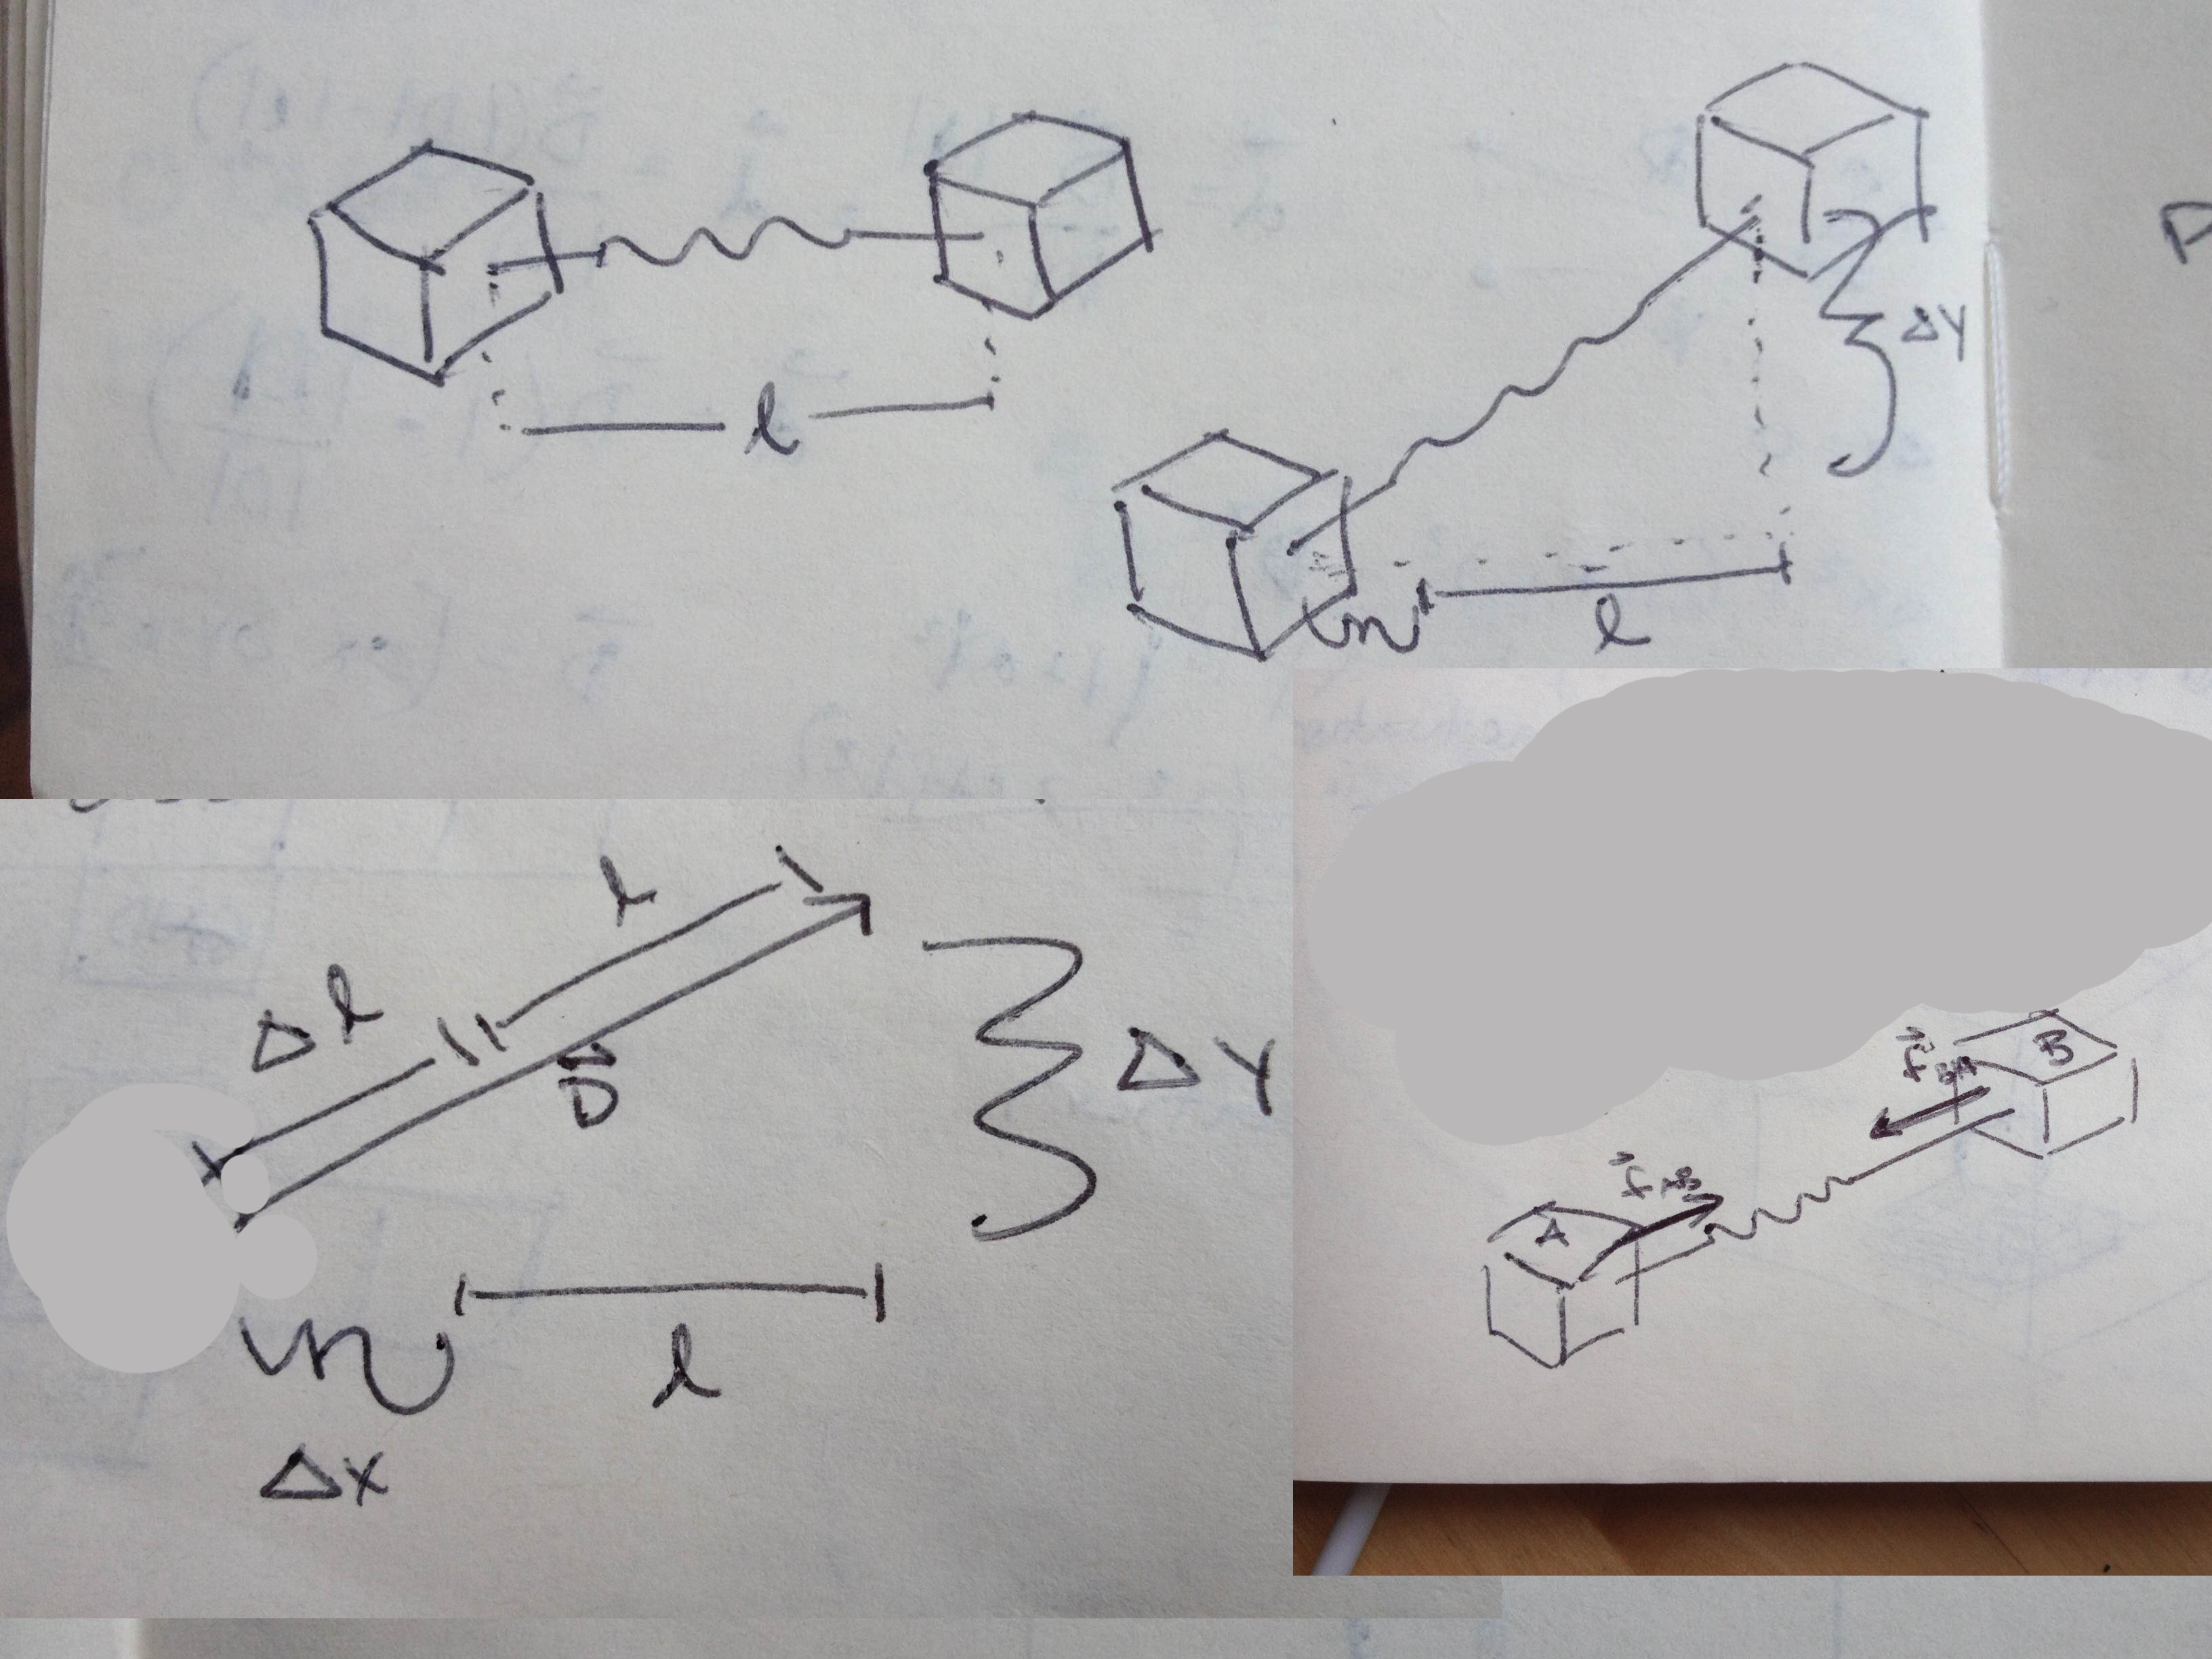
\includegraphics[width=\linewidth]{helloWorldSpringSetup.png}
%  \caption{REPLACE THIS Adjacent cells A and B connected with nominal displacement $\vec{\ell}$ \textbf{(A)}.  The cells are additionally displaced by $\Delta x$ and $\Delta y$ \textbf{(B)}. $\vec{f}_{AB}$ and $\vec{f}_{BA}$ are the resulting translational spring-damper forces applied to cells A and B, respectively \textbf{( C )}.}
%  \label{fig: helloWorldSpringSetup}
%\end{figure}
%
%
%The stiffness $k$ and damping coefficient $d$ of the springs and dampers are determined from the material properties of the two cells.  In the case that the two cells have different stiffnesses, a composite stiffness is calculated according to:
%
%\[ k = \frac{2k_Ak_B}{k_A + k_B} \]
%
%which is equivalent to two springs of half length in series.  Similarly, a composite damping coefficient is calculated by:\\
%
%\[ d = \frac{2d_Ad_B}{d_A + d_B} \]
%
%In addition to $\vec{f}_{AB}$, an equal and opposite force, $\vec{f}_{BA}$, is applied to cell B by the spring damper system (Fig \ref{fig: helloWorldSpringSetup} C):
%
%\[ \vec{f}_{BA} =  -\vec{f}_{AB}\]
%
%In addition to translational forces, neighboring cells apply torques to each other.  These torques result in rotational motion of a cell about its center of mass.  More on that soon.
%
%%\begin{figure}
%%  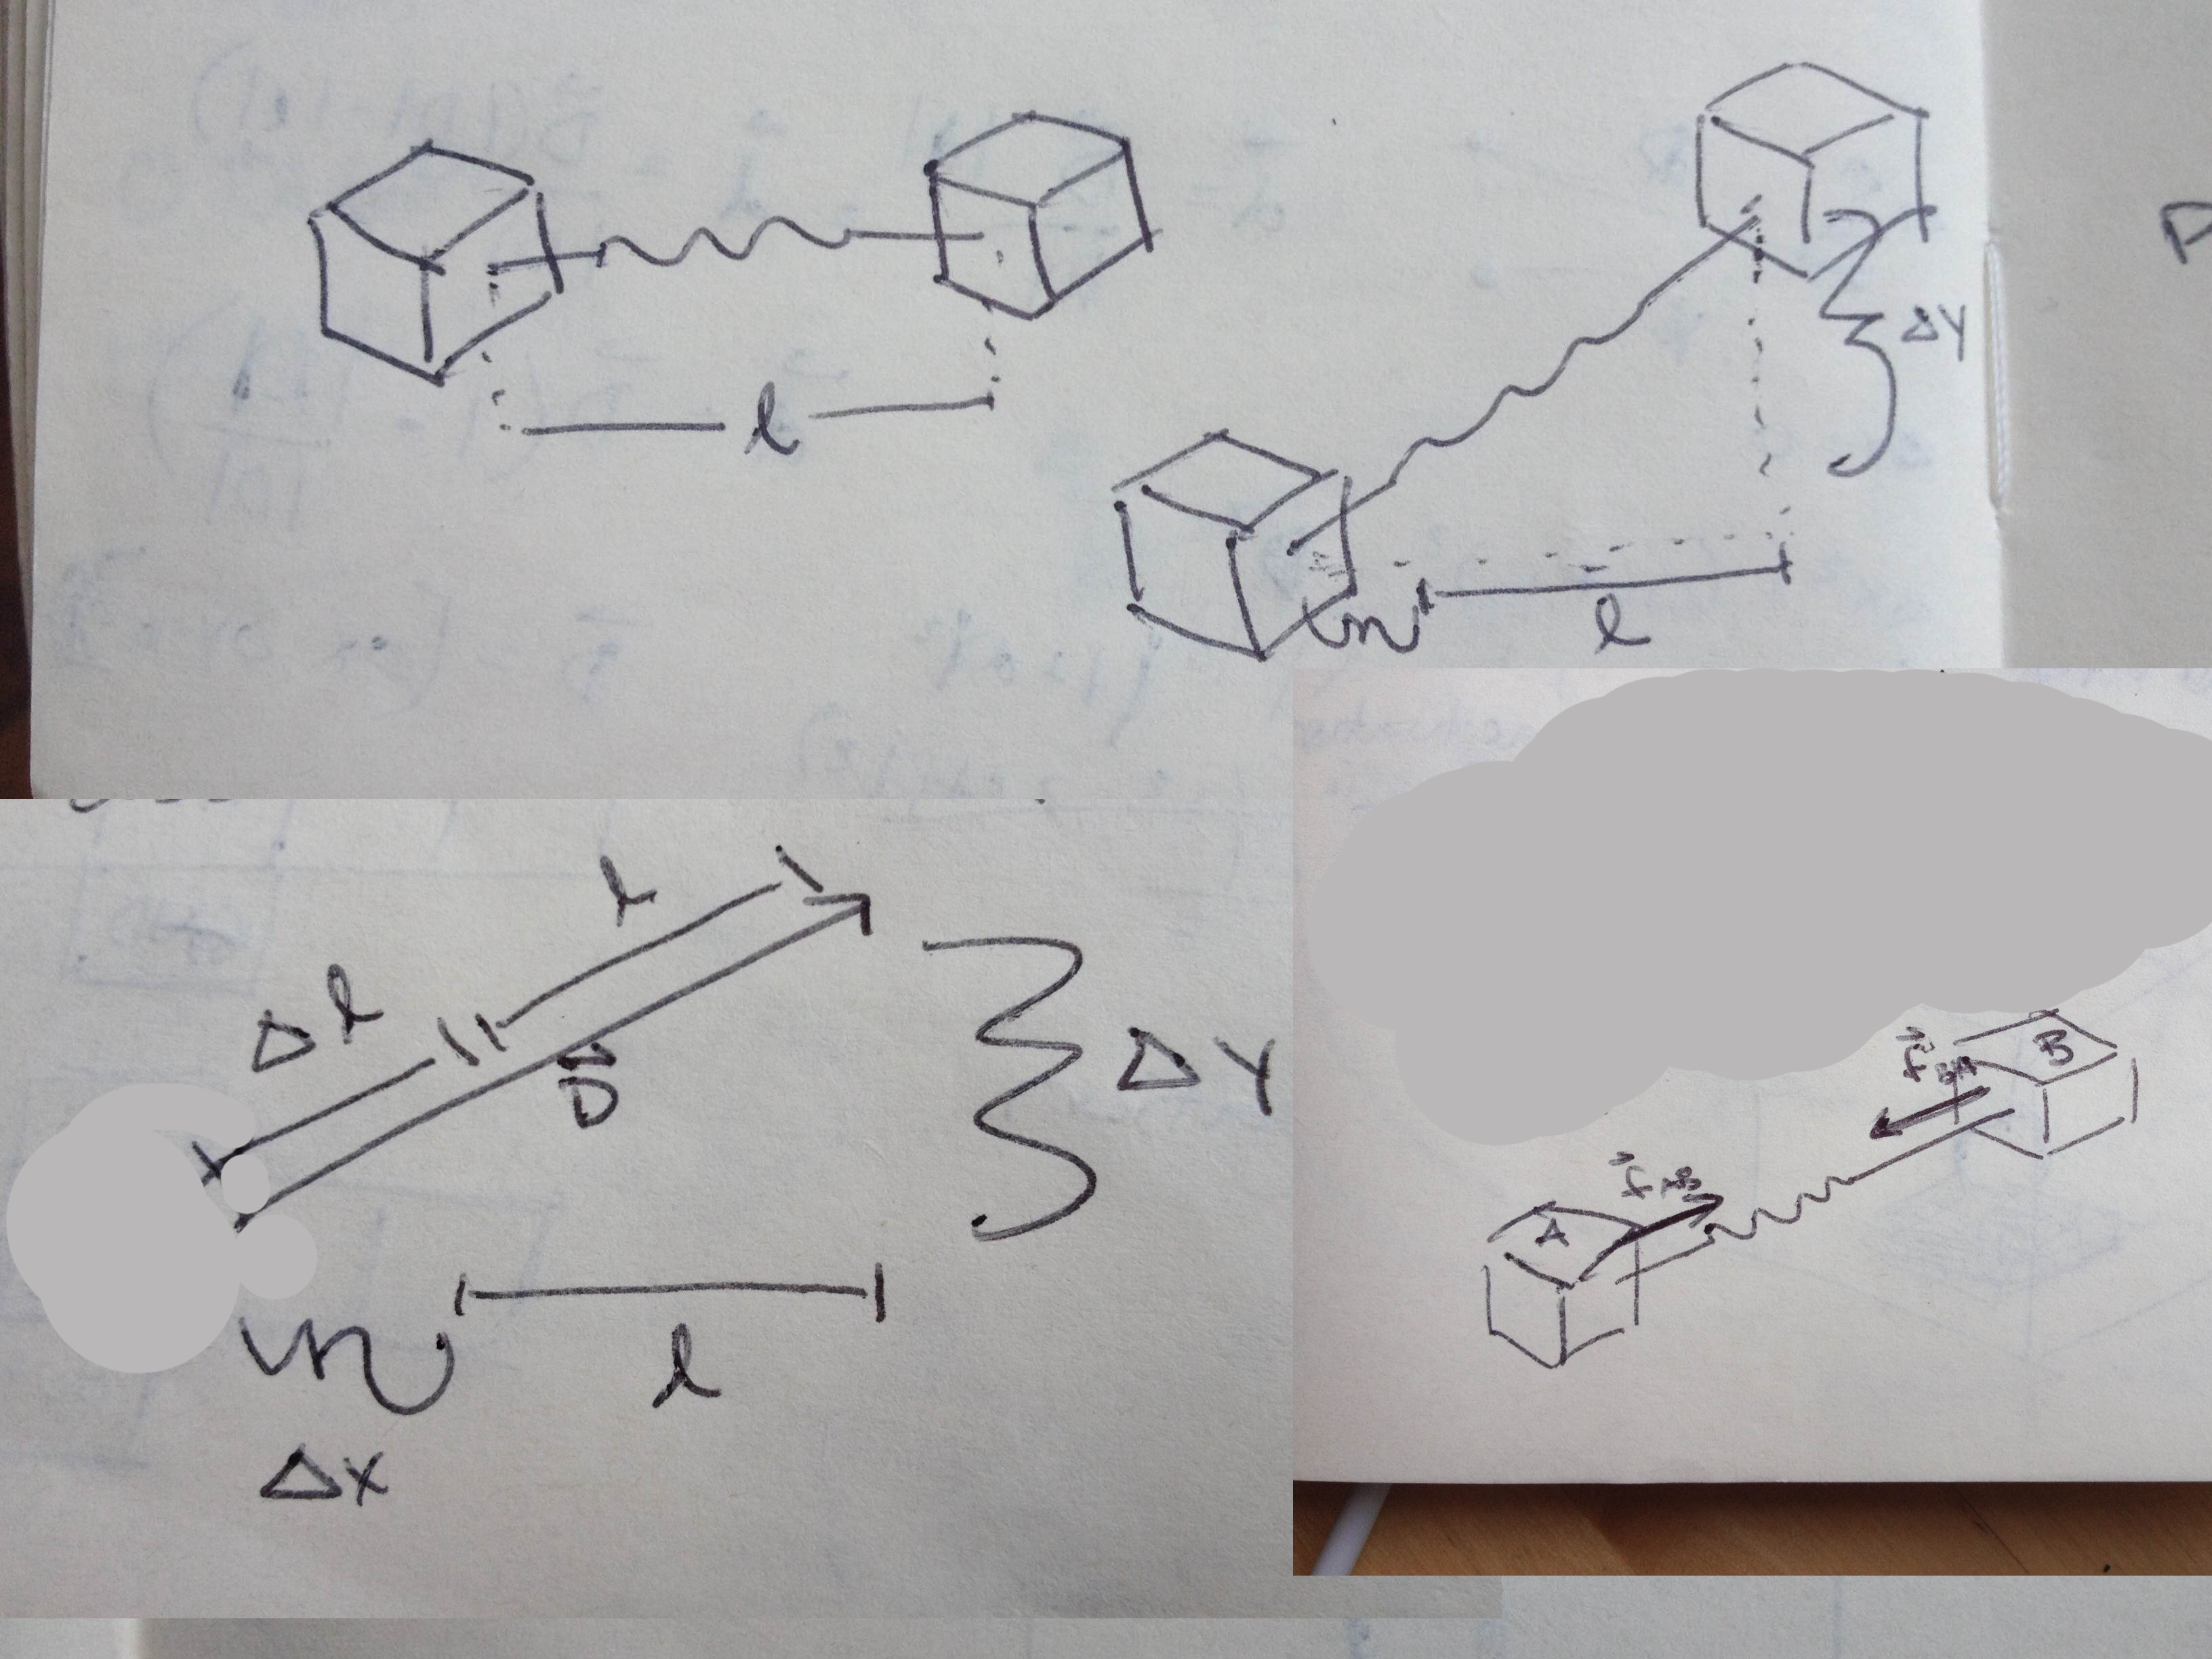
\includegraphics[width=\linewidth]{helloWorldSpringSetup.png}
%%  \caption{REPLACE THIS Cubes A and B connected by spring with nominal displacement $\ell$ \textbf{(A)}.  The cells are further displaced by $\Delta x$ and $\Delta y$ \textbf{(B)}. Spring displacement $\Delta \ell$ along $\vec{D}$ \textbf{�}.  $\vec{f_{AB}}$ is the translational spring resulting force applied to cell A by the spring attached to cell B, force of gravity, $f_g$, also indicated \textbf{(D)}.}
%%  \label{fig: helloWorldSpringRotSetup}
%%\end{figure}
%
%
%\section{Rotational Forces}
%
\section{Time Integration}

For linear systems, explicit forward time integration can be achieved using a variety of methods, each with associated error and computational cost.  The simplest and most computationally efficient approach is forward Euler:\\

\[ \vec{v}_{t+1} = \vec{v}_{t} +  \vec{a}_{t}\Delta t\]
\[ \vec{p}_{t+1} = \vec{p}_{t} +  \vec{v}_{t}\Delta t\]


Verlet integration requires storing the previous two position calculations (at time t and t-1) in order to calculate the next position:

\[ \vec{p}_{t+1} = 2\vec{p}_{t} - \vec{p}_{t-1} +  \vec{a}_{t}\Delta t^2\]
\[ \vec{v}_{t+1} = \dfrac{\vec{p}_{t+1} - \vec{p}_{t}}{\Delta t}\]

Higher order methods such as Runge-Kutta (RK4) reduce error further, but require multiple calculations in order to solve for a single time step.

 \subsection{Translational Time Integration}
 \subsection{Rotational Time Integration}


\section{Electronic Simulation}\label{sec:electronicSim}

%\section{Deviations from Reality}
%
%\subsection{Volume Preservation}
%
%Poisson's ratio $v$
%
%\begin{figure}
%  \includegraphics[width=\linewidth]{SolidMechanicsReality.png}
%  \caption{Deviation from reality in simple \textit{function} simulation.  Some coupling between degrees of freedom is expected, for example, compression on one axis will result in expansion along other, unloaded axes.}
%  \label{fig:SolidMechanicsReality}
%\end{figure}
%
%In reality, the degrees of freedom illustrated in Fig \ref{fig:SolidMechanicsDOF} are not completely orthogonal from one another.  For example, compression along one axis of a solid will cause some degree of expansion along the unloaded axes (Fig \ref{fig:SolidMechanicsReality}).  For now, I have ignored these effects.



}
